\documentclass[12pt]{article}
\usepackage[a4paper]{geometry}
\usepackage[pdftex]{hyperref}
\usepackage[german]{babel}
\usepackage[utf8]{inputenc}
\usepackage{csquotes}
\usepackage{amssymb}
\usepackage{graphicx}
\usepackage{multicol}
\usepackage{amsmath}
\usepackage{enumitem}
\usepackage{tabularx}
\usepackage{vwcol}
\usepackage{fancyhdr}
\usepackage{indentfirst}
\usepackage{polynom}

\geometry{
  headheight=14px,
  left=2.54cm,
  right=2.54cm,
  bottom=2cm,
  top=2cm
}

% For horizontally centering text in Y column
\newcolumntype{Y}{>{\centering\arraybackslash}X}

\setlength{\parindent}{0cm}

\setlength{\marginparsep}{1 cm}
\setlength{\topmargin}{-0.6in}
\setlength{\textheight}{9.5in}
\pagestyle{fancy}

% German-style quotation marks %
\MakeOuterQuote{"}

% Typesetting differential operator %
\providecommand\d{}
\renewcommand{\d}[1]{\:\mathrm{d}{#1}} 

% For vertical centering text in X/Y column
\renewcommand\tabularxcolumn[1]{m{#1}}

\polyset{%
   style=C,
   delims={\big(}{\big)},
   div=:
}

\fancypagestyle{firstpage}{%
  \lhead{\bf Staatliche Studienakademie Dresden\\
Studienrichtung: Informationstechnologie}
  \rhead{\bf Datum: 13.02.2020}
}

\cfoot{\thepage\ of \pageref*{LastTask}}


\begin{document}

\thispagestyle{firstpage}

\begin{flushright}
Anzahl der Klausurblätter: \pageref*{LastTask}
\end{flushright}

Klausur im Lehrgebiet: Algebra/Analysis\\

Teilgebiet: Analysis \\

Modulcode: 3MI-MATHE-10 \\

Lehrender: Andre Wachsmuth \\

Semester: 1 \\

\begin{vwcol}[widths={0.4,0.4,0.2},sep=0cm, justify=flush,rule=0pt,indent=4em]
Name:\\
Vorname:\\
SG:
\end{vwcol}

\bigskip
\bigskip
\bigskip
Bearbeitungszeit: 40 min \\

Zugelassene Hilfsmittel: 1 handbeschriebenes A4-Blatt \\

\textbf{Es dürfen keine eigenen Zusatzblätter abgegeben werden.} \\

\textbf{Verwenden Sie auch die Blattrückseiten für Antworten! Markieren Sie deutlich, zu welcher Frage die auf Rückseiten gegebenen Antworten gehören.} \\

\textbf {Der Rechengang muss eindeutig und vollständig ersichtlich sein!} \\

Punkteverteilung:

\bigskip

\begin{tabularx}{\textwidth}{l|Y|Y|Y|Y|Y|Y}
Aufgabe        & 1 & 2 & 3 & 4  & Zusatz & Summe \\ [1ex] \hline
Soll-Punktzahl & 7 & 8 & 8 & 9 & 2      &       \\ [3ex]
Ist-Punktzahl  &   &   &   &    &        &       \\ [3ex]
\end{tabularx}

\newpage
\section* {Aufgabe 1}

\begin{center}
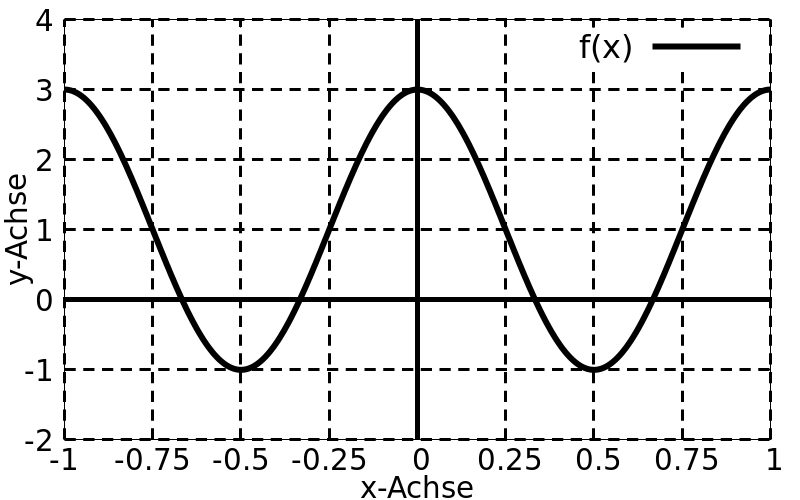
\includegraphics[width=0.95\textwidth]{grid.png}
\end{center}

\begin{enumerate}[label=(\alph*)]
\item (2P) In der oberen Skizze ist die Funktion $f(x)$ dargestellt. Es handelt sich um eine transformierte Kosinusfunktion. Lesen Sie für $f(x)$ folgende Eigenschaften ab:
\begin{itemize}

\bigskip

\item Amplitude:

\bigskip
\bigskip

\item Periode:

\bigskip
\bigskip
\bigskip

\end{itemize}
\item (3P) Finden Sie für $f(x)$ eine mögliche Funktionsgleichung! \\

\bigskip

$f(x)=$

\bigskip
\bigskip
\bigskip

\item (2P) Tragen Sie in die Skizze die Taylorentwicklung 2. Grads von $f$ an der Stelle $x_0=0{,}5$ ein!

\end {enumerate}

\newpage
\section* {Aufgabe 2}

Eine auf ganz $\mathbb{R}$ definierte Funktion $f$ lässt sich zerlegen in die Summe aus einem achsensymmetrischen Anteil $f_a$ und einem punktsymmetrischen Anteil $f_p$. Es gilt:

\begin{align*}
&f_a(x) = \frac{f(x)+f(-x)}{2}\\
&f_p(x)= \frac{f(x)-f(-x)}{2}\\
\end{align*}

\begin{enumerate}[label=(\alph*)]

\item (2P) Geben Sie eine Funktionsgleichung für den "Cosinus Hyperbolicus" an, definiert als der achsensymmetrische Anteil der Exponentialfunktion $e^x$!

\bigskip
\bigskip
\bigskip
\bigskip
\bigskip
\bigskip
\bigskip
\bigskip

\item (3P) Ermitteln Sie von $f(x) = (x+1)^2$ den punktsymmetrischen Anteil!

\bigskip
\bigskip
\bigskip
\bigskip
\bigskip
\bigskip
\bigskip
\bigskip
\bigskip
\bigskip
\bigskip
\bigskip

\item (3P) Zeigen Sie, dass $f_p$ für jede Funktion $f$ tatsächlich punktsymmetrisch ist, d.h. dass $f_p(-x) = -f_p(x)$ gilt!


\end{enumerate}

\newpage
\section* {Aufgabe 3}

Wir betrachten die Taylorreihe der Funktion $f(x) = \ln(x+1)$ an der Stelle $x_0=0$.

\begin{enumerate}[label=(\alph*)]

\item (2P) Geben Sie die 1. und 2. Ableitung von $f$ an!

\bigskip

$f'(x) = $ \\
\bigskip \\
$f''(x) = $
\bigskip
\bigskip

\item (3P) Geben Sie die Taylorentwicklung 2. Grads von $f$ an!

\bigskip
\bigskip

$\ln(x+1) \approx \hspace{2cm}   + \hspace{2cm} \cdot \hspace{1mm} x + \hspace{2cm} \cdot \hspace{1mm} x^2$
\bigskip
\bigskip
\bigskip
\bigskip


\item (3P) Die Folge der Koeffizienten $a_n$ der Taylorreihe lautet $a_n=\frac{(-1)^{n+1}}{n}$. Ermitteln Sie den Konvergenzradius R!

\bigskip

$R=1/\lim_{n\to \infty} |\frac{a_{n+1}}{a_n}| = $

\end{enumerate}

\newpage
\section* {Aufgabe 4}

Gegeben sei die inhomogene DGL

$$2y''-6y' = \frac{x^3-3x^2-x+3}{x^2-2x-3}$$

Durch Termumformung lässt sich zeigen:

$$\frac{x^3-3x^2-x+3}{x^2-2x-3} = x-1$$


\begin{enumerate}[label=(\alph*)]

\item (3P) Beweisen Sie die Termumformung mittels Polynomdivision!

$(x^3-3x^2-x+3)\div(x^2-2x-3) =$


\bigskip
\bigskip
\bigskip
\bigskip
\bigskip
\bigskip
\bigskip
\bigskip
\bigskip

\item (3P) Lösen Sie die homogene DGL $2y''-6y'=0$ mittels der charakteristischen Gleichung!

\bigskip
\bigskip
\bigskip
\bigskip
\bigskip
\bigskip
\bigskip
\bigskip
\bigskip

\item (3P) Prüfen Sie durch Einsetzen, ob $y=\frac{x}{9}-\frac{x^2}{12}$ eine Lösung der obigen inhomogenen DGL ist!

\end{enumerate}

\newpage
\section*{Zusatzaufgabe (2P)}

Die sogenannte quellenfreie d'Alembertsche Wellengleichung, welche etwa die Ausbreitung von Schall oder Wasserwellen beschreibt, lautet:

$$\Box u = 0$$


Dabei ist $\Box$ der sogenannte d'Alembert-Operator, welcher definiert ist als:

$$\Box = \frac{1}{c^2}\frac{\partial^2}{\partial t^2} - \frac{\partial^2}{\partial x^2}$$

Hierbei ist $c$ die Ausbreitungsgeschwindigkeit. Zeigen Sie, dass $u(x,t) = \sin(x+ct)$ die Wellengleichung erfüllt!

\label{LastTask}

\newpage

\begin{center}
{\bf {\large Musterlösung}}
\end{center}

\begin{center}
{\bf {\large Klausur Analysis (3IT19, 3MI19) - 13.02.2020}}
\end{center}

\begin{center}
\textbf{Jeder Anführungspunkt entspricht einem erteilten Bewertungspunkt.} 

Ist ein Rechenschritt falsch, werden für darauf basierende Rechnungen Punkte erteilt (Folgefehler), es sei denn, die Rechnung wird dadurch wesentlich vereinfacht. 
\end{center}

\begin{enumerate}

% Task 1
\item
\begin{enumerate}

\item
\begin{itemize}
\item Amplitude 2
\item Periode 1
\end{itemize}

\item $f(x) = 2\cdot\cos(2\pi x) + 1$
\begin{itemize}
\item Für den Vorfaktor ($2$)
\item Für den Koeffizient im Argument ($2\pi$)
\item Für den Summanden ($+1$)
\end{itemize}

\item 
\begin{itemize}
\item Bei $x=0{,}5$ ist eine
\item nach oben geöffnet Parabel eingezeichnet, deren Minima den Graph dort berührt
\end{itemize}

\end{enumerate}

% Task 2
\item
\begin{enumerate}

\item
\begin{itemize}
\item $\cosh(x) = \frac{f(x)+f(-x)}{2}$
\item $\cosh(x) = \frac{e^x+e^{-x}}{2}$
\end{itemize}

\item
\begin{itemize}
\item $f_p(x) = \frac{1}{2} ((x+1)^2-(-x+1)^2)$
\item $ = \frac{1}{2} (x^2+2x+1-(x^2-2x+1))$
\item $ = 2x$
\end{itemize}

\item
\begin{itemize}
\item $2f_p(-x) = f(-x)-f(x)$
\item $-2f_p(x) = -(f(x)-f(-x)) = f(-x)-f(x)$
\item Also $f_p(-x) = -f_p(x)$, dies war zu beweisen 
\end{itemize}

\end{enumerate}

% Task 3

\item
\begin{enumerate}

\item
\begin{itemize}
\item $f'(x) = \frac{1}{x+1}$
\item $f''(x) = -\frac{1}{(x+1)^2}$
\end{itemize}

\item
\begin{itemize}
\item $f(0)=\ln(0+1)=0$
\item $f'(0)=\frac{1}{0+1}=1$
\item $f''(0)/2=-\frac{1}{2(0+1)^2} = -\frac{1}{2}$
\end{itemize}

\item
\begin{itemize}
\item $R = 1/\lim_{n \to \infty} \left\{|\frac{(-1)^{n+2}}{n+1} \cdot \frac{n}{(-1)^{n+1}}|\right\}$
\item $R = 1/\lim_{n \to \infty} \frac{n}{n+1}$
\item $R = 1/1 = 1$
\end{itemize}

\end{enumerate}

% Task 4

\newpage

\item 
\begin{enumerate}

\item
\[\polylongdiv{x^3-3x^2-x+3}{x^2-2x-3}\]

\item 
\begin{itemize}
\item $2\lambda^2-6\lambda = 0$
\item $\lambda = 0 \lor \lambda = 3$
\item $y(x) = C_1 + C_2 e^{3x}$
\end{itemize}

\item 
\begin{itemize}
\item $y' = \frac{1}{9}-\frac{1}{6}x, y'' = -\frac{1}{6}$
\item $2y'' - 6y' = -\frac{1}{3} - \frac{2}{3} + x = x -1$
\item $\implies$ Die gegebene Funktion ist Lösung der inhomogenen DGL
\end{itemize}

\end{enumerate}

\end{enumerate}

\textbf{Zusatzaufgabe}

\begin{itemize}
\item $u_{tt} = -c^2\sin(x+ct)$, $u_{xx} = -\sin(x+ct)$
\item $u_{tt}/c^2 - u_{xx} = -\sin(x+ct) - (-\sin(x+ct)) = 0$
\end{itemize}


\end{document}
